\documentclass[12pt, titlepage]{article}

\usepackage{booktabs}
\usepackage{tabularx}
\usepackage{hyperref}
\usepackage{float}
\usepackage{dblfloatfix} 
\usepackage{graphicx}
\hypersetup{
    colorlinks,
    citecolor=black,
    filecolor=black,
    linkcolor=black,
    urlcolor=blue
}
\usepackage[round]{natbib}

\title{SE 3XA3: Software Requirements Specification\\Sokoban}

\author{Team 13, The Box Group
		\\ Gurpartap Kaler (kalerg1)
		\\ Freddie Yan (yanz20)
		\\ Sagar Thomas (thomas12)
}

\date{\today}

\begin{document}

\maketitle
\pagenumbering{roman}
\tableofcontents
\listoftables
\listoffigures
\begin{table}[!b]
\caption{\bf Revision History}
\begin{tabularx}{\textwidth}{p{3cm}p{2cm}X}
\toprule {\bf Date} & {\bf Developer} & {\bf Revision Notes} \\
\midrule
\\
October 3, 2018 & Sagar Thomas & Project Drivers (Revision 0)\\
October 3, 2018 & Gurpartap Kaler & Functional Req. (Revision 0)\\
October 4, 2018 & Sagar Thomas & Project Constraints (Revision 0)\\
October 4, 2018 & Freddie Yan & Non-Functional Req. (Revision 0)\\
October 4, 2018 & Gurpartap Kaler & Project Issues (Revision 0)\\
\\
\bottomrule
\end{tabularx}
\end{table}

\newpage

\pagenumbering{arabic}

This document describes the requirements for Sokoban. The template for the Software
Requirements Specification (SRS) is a subset of the Volere
template~\citep{RobertsonAndRobertson2012}.  If you make further modifications
to the template, you should explicitly state what modifications were made.

\section{Project Drivers}

\subsection{The Purpose of the Project}
\subsubsection{The User Business or Background of the Project Effort}

This project is about recreating the open-source game: Sokoban. The motivation for this project to redevelop Sokoban so that it is capable of running on as many devices as possible so that users can relive the experience of playing one of the greatest classics of all time.

\subsubsection{Goals of the Project}

The goal of this project is to redevelop Sokoban using proper software development practices to create a much more cohesive experience to the user. 

\subsection{The Client, the Customer, and other Stakeholders}

\subsubsection{The Client}
N/A - See Customers

\subsubsection{The Customers}

The customers for this game/the intended audience is anyone who has access to a computer. As with the nature of arcade games, the description of someone who would play this game can be anyone from a child looking for some entertainment to an adult looking to relive their childhood.

\subsubsection{Other Stakeholders}

\begin{itemize}
    \item General Public/Users - 
    These are the main users intended to use the product after release. They require little to no understanding of the project itself however, should be able to use the product.
    \item The Box Group - Current development team: As the developers of the game, we hold responsibilities to ensure that this game meets the goals that we planned. All members should have a clear understanding of everything that goes on in the project. Any conflicts among us will be resolved through group discussions until a resolution is reached or a majority vote.
    \item Teaching Staff - As the overseers of the project, they have a basic understanding of it and keep track of the progress through various milestones.
\end{itemize}

\subsection{Users of the Product}
\subsubsection{The Hands-On Users of the Product}
The Hands-On Users of the product are the customers as described above. These people can be described as children of different age groups or adults in their early 20s to 30s. As part of the younger generation, they have a very high degree of technical skill in using a computer.
\subsubsection{Priorities Assigned to Users}
\begin{itemize}
    \item Key Users: The client/customers - namely the population of people who are adept at using computers as well as in need of entertainment in the form of a game or people looking for a nostalgic experience of a classic game.
    \item Secondary Users/Unimportant Users - Everyone who doesn't fall into the first category of Key Users.
\end{itemize}

\subsubsection{User Participation}
The only form a participation the users will have to provide is playing the game after release.

\subsubsection{Maintenance Users and Service Technicians}

It is possible to release beta builds of the game and have select users test new game features before its released the the rest of the users. Aside from that, users will be able to report any bugs they find while playing the game so in that aspect, all users are potential Maintenance Users.

\section{Project Constraints}

\subsection{Mandated Constraints}
\subsubsection{Solution Constraints}
\begin{itemize}
    \item Description: The game should be implemented and ran in Python 3.6.1 or greater 
    \\\\\
    Rationale: The underlying library powering the game, \href{https://www.pygame.org/news}{PyGame}, requires Python 3.6.1 or greater for optimal speed and functionality 
    \\\\
    Fit criterion: The install script for the game will check for a acceptable Python installation on the user device and install if necessary.
    \item The game shall be playable without an active internet connection
    \\\\
    Rationale: As one of the main goals of this game is to be playable at any time on any device, it is essential that the game is playable offline.
    \\\\
    Fit criterion: The game will not use any code that would request online resources or services after installation with the exception of checking for updates. The game will also be tested extensively in an environment without internet.
    
\end{itemize}

\subsubsection{Implementation Environment of the Current System}
The product is to be installed and ran on any popular operating system such as Linux, MacOS or Windows. In terms of physical environments, the product should be able to run on all modern PC architectures (32-bit, 64-bit, ARM etc.) that have the capability to run Python.

\subsubsection{Partner or Collaborative Applications}

This product does not have any partner or collaborative applications as it is completely a standalone product. The only direct dependencies would be the OS and the Python runtime.

\subsubsection{Off-the-Shelf Software}

The product uses the open-source library PyGame to power the entire game. Pygame handles all rendering to the screen as well as exposing the input stream from the user in a easy-to-use API. We also use PyUnit, a free testing framework bundled with Python.

\subsubsection{Anticipated Workplace Environment}

The anticipated workplace environment would be a simple setup of a keyboard and mouse/trackpad in any location.

\subsubsection{Schedule Constraints}
The main deadline is that this project must be complete before the end of the current term (December 2018). Throughout the term, there will be various deadlines and milestones to adhere to which can be found in our
\href{https://gitlab.cas.mcmaster.ca/kalerg1/se3xa3/tree/master/Sokoban-Game/ProjectSchedule}{Project Schedule}.

\subsubsection{Budget Constraints}

N/A - No monetary budget for this project

\subsection{Naming Conventions and Terminology}
\subsubsection{Definitions of All Terms, Including Acronyms, Used in the Project}
\begin{tabularx}{\textwidth}{|X|X|}
    \hline
     Terms/Acronyms & Definition   \\
     \hline
     OS & Operating System \\
     \hline
     User & A person that is the intended target of the product \\
     \hline
     UML & Unified Modelling Language \\ 
     \hline
     FR & Functional Requirement \\ 
     \hline
     Sokoban & Name of the product/game in development \\
     \hline
     DR & Data Requirement \\ 
     \hline
     Gradle & Build and Dependency manager tool for Java \\
     \hline
     OP & Original Project - refers to the open-source project that is being redeveloped by this project \\ 
     \hline
     
\end{tabularx}
\subsection{Relevant Facts and Assumptions}
\subsubsection{Facts}
The OP on Github was around 441 lines of code written in Java. The OP requires Gradle to be installed on the user's machine in order to run it, which is fairly difficult for someone without a technical background to do. In this project, the ease of installation should be a focus as well.

\subsubsection{Assumptions}
\begin{itemize}
    \item It is expected that the user will be using one of either Linux, MacOS or Windows when playing the game.
    \item It is expected that Python is installed on the user's computer or the user is able to install the correct version of Python given appropriate instructions from the game installer.
    \item It is expected that the user has a basic understanding of computers and is familiar with using a mouse/keyboard.
\end{itemize}

\section{Functional Requirements}

\subsection{The Scope of the Work and the Product}

\subsubsection{The Current Situation}
The OP exists on GitHub, and it is called \href{https://github.com/gaborbata/boxbot4k}{boxbot4k}. This implementation of Sokoban is in Java, however we are choosing to re-implement it into Python. We intend to keep the same logic as the original game, but make it in a different language. Furthermore, methods and modules will be re-added to our implementation if they prove to be effective. Finally, we wish to optimize the game, and add more features.

\subsubsection{The Context of the Work}
Deliverables:
\begin{itemize}
    \item Final Documentation
    \begin{itemize}
        \item Problem Statement
        \item Development Plan
        \item Requirements Document
        \item Design Document
        \item Test Plan
        \item Test Report
    \end{itemize}
    \item Final Source Code
\end{itemize}
\noindent Deadlines:
\begin{itemize}
    \item Requirements Document Revision 0 - October 5, 2018
     \item Proof of Concept Demonstration - Week of October 15, 2018 
     \item Test Plan Revision 0 - October 26, 2018
      \item Design \& Documentation Revision 0 - November 9, 2018
      \item Revision 0 Demonstration - Week of November 12, 2018
      \item Final Demonstration Revision 1 - Week of November 26, 2018
      \item Final Documentation Revision 1 - December 5, 2018 
\end{itemize}

\subsubsection{Work Partitioning}

Work Partitioning is already shown in our Gantt Chart, in our \href{https://gitlab.cas.mcmaster.ca/kalerg1/se3xa3/tree/master/Sokoban-Game/ProjectSchedule}{Project Schedule} folder.

\subsection{The Scope of the Project}
\subsubsection{Product Boundary}
\begin{figure} [H]
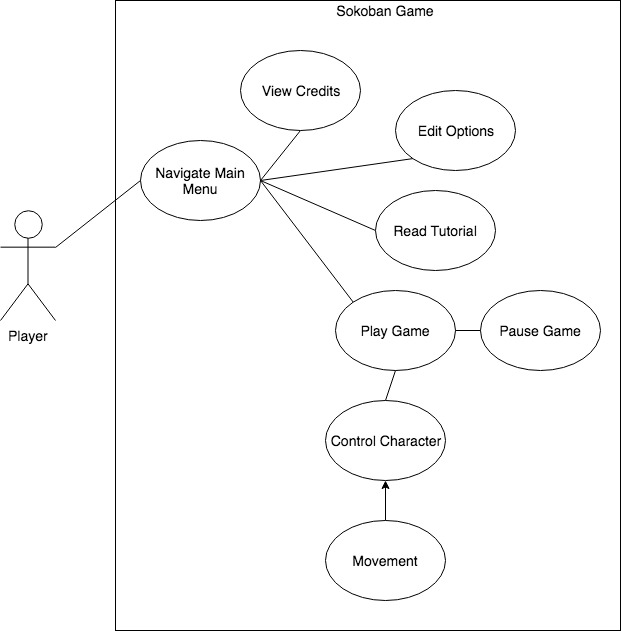
\includegraphics[scale=0.5]{Sokoban.jpg}
\caption{Sokoban Game UML Use Case Diagram}  
\end{figure}

\subsubsection{Product Use Case List}
\subsubsection{Individual Product Use Cases}

\subsection{Functional and Data Requirements}

\subsubsection{Functional Requirements}

\begin{itemize}
\item Requirement Number: FR1 

The product should work offline. 

Rationale: Users should be able play this game at any time.

\item Requirement Number: FR2

The product should be packaged, with all files intact.

Rationale: This will make it easier for the user to download the file from the internet.

\item Requirement Number: FR3

The size of the game window should be adjustable

Rationale: Sokoban will not take the whole screen to play, however, it should be the users option how to experience the game.

\item Requirement Number: FR4

The character shall only move one cell, with every reasonable input from the user (key up, key down, key left, key right).

Rationale: The movement of the character should always under player's control, one cell at a time.

\item Requirement Number: FR5

The user should be able to undo their characters movement, and the actions that the character takes.

Rationale: This will allow the user to undo any mistakes made during the maze, so they do not need to restart the game.

\item Requirement Number: FR6

Sokoban shall contain 10 different mazes, that have different difficulty levels.

Rationale: This will allow the user to progress through the game of Sokoban.

\item Requirement Number: FR7

The character of the game should not be able to go through any walls of the maze.

Rationale: The user should not be able to move the character through the walls of the maze, as this is not possible.

\item Requirement Number: FR8

When the character of the game is beside a box, and the character travels in the same direction as the box, the character and the box should move one space.

Rationale: The user should be able to successfully push the box around the maze.

\item Requirement Number: FR9

When all boxes are placed in their designated locations, the game should enter a winning condition.

Rationale: The user should be able to win.

\item Requirement Number: FR10

The boxes should be able to be moved outside the designated location, even after the user moved them there.

Rationale: The user should be able to move the boxes outside their designated location, in case that area is needed to move another box to its designated location.

\item Requirement Number: FR11

The box should not be able to go through any walls of the maze.

Rationale: The user should not be able to move the boxes through the walls of the maze, as this is not possible.

\item Requirement Number: FR12

The user interface must have a link to the tutorial/user manual.

Rationale: To help the user interface and play Sokoban.

\item Requirement Number: FR13

The tutorial/user manual should include pictures or short videos explaining steps.

Rationale: The user should be able to understand how to play the game, even without reading, accessibility to younger audience.

\item Requirement Number: FR14

When the user enters a game winning condition for a maze, the product shall start the next level.

Rationale: The user should be able to play the next level, when they win the current one.

\item Requirement Number: FR15

When the user enters the last game winning condition for a maze, the game shall show a winning screen and restart the game.

Rationale: The user should know when they win all the stages of the game.

\end{itemize}

\subsubsection{Data Requirements}

\begin{itemize}
    \item Requirement Number: DR1

Sokoban should not read or write to any of the users files on the computer it is installed on.

Rationale: The program should not need access to any of the user's personal files.

\end{itemize}

\section{Non-functional Requirements}

\subsection{Look and Feel Requirements}
\subsubsection{Appearance Requirements}

\begin{itemize}
    \item Requirement Number: NF1
    
The product shall display the company logo, name, and the license of the product upon starting.

Rationale: The user should know who created the game.
    \item Requirement Number: NF2
    
After Sokoban is opened and before user starts, it should provide a start button which is centered in the game window, with a background of a sample maze from the product.

Rationale: The user should be able to start the game from the main menu.
    \item Requirement Number: NF3
    
For the users' convention, the size of the window should be adjustable.

Rationale: The user should be able to use the game in any window size they want, including full screen.
\end{itemize}

\subsubsection{Style Requirements}
\begin{itemize}
    \item Requirement Number: NF4
    
When the game is running, the backgrounds of different levels shall change color and theme.

Rationale: The user should feel some sort of progression and difficulty as the colors get darker.
    \item Requirement Number: NF5
    
     The color of the character's clothing should always match with the environment.
     
    Rationale: The user should feel engaged with the character throughout the game.
\end{itemize}


\subsection{Usability and Humanity Requirements}
\subsubsection{Ease of use requirements}
\begin{itemize}
        \item Requirement Number: NF6

Sokoban shall only require the user's mouse for navigating the menu, and four keys, including up, down, left, and right to control.
     
    Rationale: This will make the game playable by a wider audience, either younger or older.
\end{itemize}


  
\subsubsection{Personalization and Internationalization requirements}

\begin{itemize}
    \item Requirement Number: NF7
    
Sokoban should only display few simple English words in the game interface.
     
    Rationale: We want our game accessible to anyone that wants to play it. Including those whose first language is not English.
    
        \item Requirement Number: NF8
    
All tutorials and menus should include graphics and pictures.
     
    Rationale: We want our game accessible to anyone that does not know any English.
\end{itemize}

\subsubsection{Learning Requirements}
\begin{itemize}
            \item Requirement Number: NF9
    
Sokoban shall include a tutorial that explains all rules for the game.
     
    Rationale: We want all users to have access to the rules if they don't know how to play. 
    
        \item Requirement Number: NF10
    
Sokoban shall include a really simple instruction manual.
     
    Rationale: We want to be straight to the point with our instruction manual, so the game is easier and quicker to learn.
\end{itemize}


\subsubsection{Understandability and Politeness Requirements}

\begin{itemize}
    \item Requirement Number: NF11
    
Sokoban shall address users of any age, gender, and race/ethnicity as the same. 
     
    Rationale: The user should not have to feel left out or targeted due to our product.
\end{itemize}



\subsection{Performance Requirements}
\subsubsection{Speed and Latency requirements}
\begin{itemize}
 \item Requirement Number: NF12
    
Anytime the user gives an input, the program shall move immediately (within 1 second) of the input.
     
    Rationale: We want the user to really feel like they are the character, so there should be no input lag.
\item Requirement Number: NF13
    
The program shall not cause the users computer to lag or hang.
     
    Rationale: We do not want Sokoban to hinder the performance of the users PC in any way.
\end{itemize}

\subsubsection{Safety-Critical requirements}

\begin{itemize}
    \item Requirement Number: NF14
    
Sokoban shall not take over any of the computers function, such as reading or writing files.
     
    Rationale: We want the users to be in control of their own computer functions at all times.
    
    \item Requirement Number: NF15
    
 Sokoban should be secure, and should not create any gaps in the current security of the system.
     
    Rationale: The user should not have to be worried about security when playing Sokoban.
\end{itemize}

\subsubsection{Precision or Accuracy requirements}
\begin{itemize}
    \item Requirement Number: NF16
    
Sokoban shall follow all inputs correctly, accurate to the direction key that the user presses (Up, Down, Left, Right).
     
    Rationale: The user should feel like they are in control of the character with their inputs.
\end{itemize}

\subsubsection{Reliability and Availability requirement}
\begin{itemize}
    \item Requirement Number: NF17
    
Sokoban should be usable 24 hours per day, 365 days per year.
     
    Rationale: The user should always be able to play Sokoban.
\end{itemize}


\subsubsection{Robustness or Fault-Tolerance Requirements}

\begin{itemize}
    \item Requirement Number: NF18
    
Sokoban shall not react or give output to any inputs out of its bounds (if a key other than the arrow keys is pressed).
     
    Rationale: If the user accidentally presses another button on the keyboard, the game should not respond and ruin the progress.
\end{itemize}


\subsubsection{Capacity requirement}

\begin{itemize}
    \item Requirement Number: NF19
    
Sokoban shall be able to accommodate one user per account per computer.  
     
    Rationale: Usually there is only one user per account on each computer.
\end{itemize}


\subsubsection{Scalability or Extensibility requirements}

\begin{itemize}
    \item Requirement Number: NF20
    
Sokoban shall be able to be downloaded unlimited amount of times from the internet onto users' computers.
     
    Rationale: The user should be able to download Sokoban on any computer, so they can use the game locally.
\end{itemize}

\subsubsection{Longevity requirements}

\begin{itemize}
    \item Requirement Number: NF21
    
Sokoban shall function for a minimum for two years, with regular maintenance.
     
    Rationale: We want Sokoban able to function until the end of our Undergraduate Software Engineering degrees.
\end{itemize}

\subsection{Operational and Environmental Requirements}
\subsubsection{Expected physical environment}

\begin{itemize}
    \item Requirement Number: NF22
    
Sokoban shall be installed as a computer application on most desktops and laptops.
     
    Rationale: The user will only be able to play Sokoban on their computer.
\end{itemize}

\subsubsection{Requirements for Interfacing with Adjacent Systems}

\begin{itemize}
    \item Requirement Number: NF23
    
Sokoban shall work on the releases of Windows, Mac OS, and Linux that are compatible with Python 3.
     
    Rationale: The user will only be able to play Sokoban on OS's that are compatible with Python 3.
    
    \item Requirement Number: NF24
    
 Sokoban shall be downloaded from the internet on all versions of internet browsers.
     
    Rationale: The user should be able to download Sokoban from any internet browser that supports downloading.
\end{itemize}

\subsubsection{Installability requirements}

\begin{itemize}
    \item Requirement Number: NF25
    
Sokoban shall be distributed as a package the user can download and install onto the computer.
     
    Rationale: The user should be able to install all of Sokoban from one package.
\end{itemize}

\subsubsection{Release Requirements}

\begin{itemize}
    \item Requirement Number: NF26
    
Each release should not cause the previous version to fail and will be offered to users on the "as-needed" basis. 
     
    Rationale: The user should be able to update his local files of Sokoban whenever they want to.
\end{itemize}

\subsection{Maintainability and Support Requirements}
\subsubsection{Maintenance requirements}

\begin{itemize}
    \item Requirement Number: NF27
    
New levels or backgrounds should be updated regularly.
     
    Rationale: In order to attract more users, we want to add new themes.
   \item Requirement Number: NF28
    
New methods/functions shall be added to Sokoban as the users suggest it.
     
    Rationale: If a majority of users want a new feature in Sokoban, we will add it to supply their demand. 
    
    \item Requirement Number: NF29
    
Sokoban should be regularly updated (once every month), to deal with any outstanding bugs or errors.
     
    Rationale: Users should not have to deal with bugs or errors in Sokoban, thus we will regularly update.
    
\end{itemize}

\subsubsection{Supportability requirements}
\subsubsection{Adaptability}

\subsection{Security Requirements}
\subsubsection{Access requirements}

\begin{itemize}
    \item Requirement Number: NF30
    
Only developers should be able check the source code of Sokoban.
     
    Rationale: Users should not be able to change the source code of Sokoban.
\end{itemize}

\subsubsection{Integrity requirements}

\begin{itemize}
    \item Requirement Number: NF31
    
Sokoban should prevent incorrect data and input from being used.
     
    Rationale: Sokoban requires no data to be used. Users should not be inputting from devices like video game controllers.
\end{itemize}



\subsubsection{Privacy requirements}

\begin{itemize}
    \item Requirement Number: NF32
    
Sokoban shall not collect any information from its users.
     
    Rationale: The users information is private and is not necessary for Sokoban to function
\end{itemize}


\subsubsection{Audit requirement}
\begin{itemize}
    \item Requirement Number: NF34
    
Sokoban shall be regularly audited every month.
     
    Rationale: The users should not have to deal with any outstanding issues of Sokoban.
\end{itemize}


\subsubsection{Immunity Requirements}

\begin{itemize}
    \item Requirement Number: NF35
    
Sokoban shall protect itself from viruses, worms, and Trojan horses, by only using relevant files.
     
    Rationale: The users computer should be secure even with Sokoban installed.
\end{itemize}

\subsection{Cultural and Political Requirements}

\subsubsection{Cultural Requirements}

\begin{itemize}
    \item Requirement Number: NF36
    
Sokoban will not use any text, images, or media that will offend the countries that use it. 
     
    Rationale: The users of Sokoban can be from any country, and we would not like to offend them.
\end{itemize}


\subsubsection{Political Requirements}

\begin{itemize}
    \item Requirement Number: NF37
    
Sokoban shall show a disclaimer explaining any similarities to any cultural or political symbols or figure is coincidental. 
     
    Rationale: Users should not have to feel offended, because that was not the intention of the product.
\end{itemize}

\subsection{Legal requirements}

\subsubsection{Compliance requirements}

\begin{itemize}
    \item Requirement Number: NF38
    
Sokoban will not violate any copyright laws.
     
    Rationale: Sokoban should not copy anyone's work.
\end{itemize}


\subsubsection{Standards requirements}
\begin{itemize}
    \item Requirement Number: NF39
    
Sokoban shall follow the MIT open license.
     
    Rationale: Sokoban should follow the MIT open license, as the OP on GitHub followed the same license.
\end{itemize}

\subsection{Health and Safety Requirements}
\begin{itemize}
    \item Requirement Number: NF40
    
Sokoban shall try to reduce the damage from the monitor to the user's eyes.
     
    Rationale: The user should not be harmed by Sokoban, or compromise the user's sleep patterns.
    
    \item Requirement Number: NF41
    
Sokoban shall not harm or dictate harm to any characters in the game

    Rationale: Young kids are potential users of the game, and they should not be exposed to violence.
\end{itemize}

\section{Project Issues}

\subsection{Open Issues}

\noindent Understanding of code structure of existing open-source project
\begin{itemize}
    \item The original project that we are working with is implemented in Java. We will have to analyze the functions to re-implement in Python.
\end{itemize}

\noindent Python Version
\begin{itemize}
    \item Currently we have not decided what version of Python to use. We have to evaluate multiple factors for both languages.
\end{itemize} 

\noindent Automated Testing
\begin{itemize}
    \item The ability to complete a fully automated test is still incomplete. Our group has to look into the feasibility of automated testing for the game.
\end{itemize}

\subsection{Off-the-Shelf Solutions}
\subsubsection{Ready-Made Products}
There are already many existing products for that have created the game of Sokoban. The are listed below:

\begin{itemize}
    \item \href{https://play.google.com/store/apps/details?id=br.com.orangevoid.sokobanfree}{Sokoban Original \& Extra: Free by Orange Void}
    \item \href{https://play.google.com/store/apps/details?id=com.gamesbykevin.sokoban}{Sokoban by Games by Kevin}
    \item \href{https://play.google.com/store/apps/details?id=org.alesapps.sokobanfree}{Sokoban Collection Free by Ales Apps}
\end{itemize}

There are many other variations of Sokoban found online. We are going to investigate these ready-made products as potential solutions, and see if they can improve our implementation.

\subsubsection{Reusable Components}
There is one particular reusable component that we can use, it is called \href{https://www.pygame.org/news}{PyGame}. PyGame is a library that helps make multimedia applications like games in Python. It will really be helpful creating Sokoban, and we can use the library to make the implementation easier. PyGame will also help because it is highly portable and is able to run on all operating systems.

\subsubsection{Products That Can Be Copied}

Some products that can be copied are listed below:

\begin{itemize}
    \item \href{https://github.com/kazantzakis/pySokoban}{pySokoban (Python)}
    \item \href{https://github.com/gaborbata/boxbot4k}{boxbot4k (Java)}
\end{itemize}

The products above are open source and available on GitHub. These products will make it easier to engineer the logic behind the game. It will also help with breaking the game down into sizable modules.

\subsection{New Problems}
\subsubsection{Effects on Current Environment}

\subsubsection{Effects on the Installed Systems}

Installing the game on the users computer can cause issues on their computer. Our game could potentially cause the users computer to hang, and freeze, if it is not optimized.

\subsubsection{Potential User Problems}

The visual effects of the game could lead to the user to become ill. To combat this, we will include a dimmed down version of the game. This will help as the colors will not be as bright and shocking to the user. Furthermore, the game might be too complicated for some of our audience. We will have to make a tutorial that is appropriate for everyone in our scope.

\subsubsection{Limitations in the Anticipated Implementation Environment That May Inhibit the New Product}

\subsubsection{Follow-Up Problems}

If the program has a bug in the future that makes in unplayable. We will try to find the bug as soon as possible and return the game back to working condition.

\subsection{Tasks}
\subsubsection{Project Planning}

The project's tasks are set by the deliverable outline for SFWRENG 3XA3. The final demonstration and documentation will need to be completed by December 5, 2018.

\subsubsection{Planning of Development Phases}

The project will be developed over the semester. There will be a Proof of Concept demonstration on the week of October 15th, 2018. After this, we will have a Revision 0 demonstration on the week of November 12th, 2018. The project is expected to be fully developed by our Revision 1 demonstration on the week of November 26th, 2018.

\subsection{Migration to the New Product}

\subsubsection{Requirements for Migration to the New Product}

Requirements will be drilled down on over time according to the priorities listen in this documentation. Furthermore, we will follow our Gantt Chart that outlines our project schedule. The product will be tested on most OS's including Windows, Mac OS, and Linux. The program will be backed up on GitLab, as well as local respositories throughout the migration. 

\subsubsection{Data That Has to Be Modified or Translated for the New System}

\subsection{Risks}

The risks of this project include that it may be too difficult to add all the extra features we would like to. For example, the feature of having different themes in the game, may require too many external libraries. We would also need to include a unique skin for each character in the game. Furthermore, testing may be difficult to automate because we do not have prior experience with it. However, another option for testing includes user testing, which is not efficient or accurate in determining that the product is bug free. User testing will help determine the functionality of our program. 

\subsection{Costs}

Effort costs will be distributed equally to each team member, and is outlined through our Gantt Chart, in our \href{https://gitlab.cas.mcmaster.ca/kalerg1/se3xa3/tree/master/Sokoban-Game/ProjectSchedule}{Project Schedule} folder. We will not need to spend any money creating the project, as long as the images and image editing software that we use remain free.

\subsection{User Documentation and Training}
\subsubsection{User Documentation Requirements}

The product will contain a tutorial menu, where the user will learn to to use the application. They will also learn how to use the features of the program, like changing the themes, turning off the game music, etc.

\subsubsection{Training Requirements}

The product will contain a tutorial level, where the user learns how to play the game.

\subsection{Waiting Room}

The functional and non-functional requirements need to be implemented in our final program. The prototype also needs to be created for the Proof of Concept demo.

\subsection{Ideas for Solutions}

Using \href{https://www.pygame.org/news}{PyGame} for can help implement our requirements much quicker. As we could reuse code that already exists. Furthermore, we can use \href{https://github.com/google/styleguide/blob/gh-pages/pyguide.md}{Google} code style for Python code, to ensure we have correct documentation.

\clearpage

\bibliographystyle{plainnat}

\bibliography{SRS}

\newpage

\section{Appendix}

\subsection{Symbolic Parameters}


\end{document}